\documentclass[a4paper, 12pt]{article}
\usepackage[top=1cm, bottom=2.1cm, left=2cm, right=2cm]{geometry}
\usepackage[utf8]{inputenc}
\usepackage{graphicx, caption}
\usepackage{float}
\usepackage{amsmath, amsfonts, amssymb, esint}
\usepackage{hyperref}
\usepackage{multicol}
\usepackage{color}
\usepackage{wallpaper}
\usepackage{array}

\CenterWallPaper{1}{./img/background.png}

\hypersetup{
    colorlinks=true,
    linkcolor=blue,
    filecolor=magenta,      
    urlcolor=cyan,
}

\definecolor{red}{rgb}{1,0,0}
\newcommand{\red}[1]{\textcolor{red}{#1}}

\newcolumntype{M}[1]{>{\centering\arraybackslash}m{#1}}

\begin{document}
    \begin{figure}
        \centering
        \href{https://ligaolimpicadeastronomia.com.br/}{
\includegraphics[scale=0.6]{./img/logos.png}}
    \end{figure}
    \begin{center}
        \begin{large}
            \textbf{Simulado -- Intensivão para a OBA}
            \linebreak \red{Gabarito}
        \end{large}
        \end{center}
    \begin{flushright}
        Material elaborado por \textbf{Iago Mendes}
    \end{flushright}

    \begin{flushleft} \begin{itemize}
        \item \textbf{Questão 1) (1 ponto)} Todas as civilizações da Antiguidade que nos deixaram registros astronômicos observaram que, além das estrelas que pareciam fixas umas em relação às outras, existiam cinco pontos luminosos que passeavam por entre as estrelas, os planetas visíveis a olho nu: Mercúrio, Vênus, Marte, Júpiter e Saturno. Os demais planetas não eram conhecidos nesta época, pois não havia telescópios. A partir da invenção do telescópio – utilizado pela primeira vez por Galileu Galilei para estudar o céu – foram identificados os demais planetas, além de diversos outros corpos celestes não observáveis a olho nu, como satélites planetários, um grande número de asteroides e cometas de baixa luminosidade. Uma primeira estrutura foi identificada no início do século XIX, o Cinturão de Asteroides, cujos componentes foram descobertos em sequência à descoberta do maior deles, Ceres (descoberto em 1801 por Giuseppe Piazzi), que, com seus 950 km de diâmetro, apesar de esférico, era pequeno demais para ser considerado um planeta. Além disso, vários outros corpos bem menores, basicamente rochosos, foram observados tendo órbitas entre Marte e Júpiter. Hoje, os astrônomos julgam que Júpiter teria impedido a formação de um planeta entre ele e Marte dando origem a este cinturão. É importante mencionar que a formação dos corpos do Sistema Solar (Sol, planetas e demais corpos) deu-se por aglutinação de corpos menores ao longo de alguns poucos milhões de anos, partindo da condensação de uma nuvem de gás e poeira primordial. Os astrônomos atualmente também concordam que existem duas outras regiões de corpos menores no Sistema Solar e até acham que estes corpos estão lá porque foram expulsos quando os planetas já estavam formados. A primeira destas estruturas, que começa logo depois da órbita de Netuno, é o assim chamado Cinturão de Kuiper, cujos corpos estão espalhados em órbitas próximas ao plano das órbitas dos planetas. À medida que nos afastamos mais ainda do Sol, as órbitas dos corpos menores vão se espalhando por uma região cada vez mais extensa, até que a cerca de 0,5 ano luz do Sol, indo até 1 ano luz, as órbitas estão tão espalhadas que encontramos corpos com órbitas em qualquer ângulo em relação ao plano das órbitas dos planetas. Esta estrutura que envolve esfericamente todo o Sistema Solar, a uma grande distância dos planetas, é chamada de Nuvem de Oort. Para se ter uma ideia do quão longe significa 0,5 ano luz de distância, Netuno está a apenas cerca de 4 horas (!) luz e Plutão a pouco mais de 5 horas luz do Sol. Os corpos constituintes do Cinturão de Kuiper e da Nuvem de Oort são, em sua grande maioria, formados de constituintes mais leves, como água, metano e, em menor quantidade elementos rochosos, ou seja, o que é chamado de gelo sujo. Acredita-se, inclusive, que a origem dos oceanos terrestres teria sido um bombardeamento por cometas. Na verdade, Jan Hendrik Oorte Gerard Peter Kuiper ao proporem, no início da década de 50 do século passado, as estruturas que terminaram por receber seus nomes, estavam pensando nesta outra classe de corpos menores, os cometas, já então com grande número de ocorrências registradas e estudadas à época. Assim, cometas de período da ordem do Cometa Halley, isto é de ``curto período'', com órbitas próximas ao plano da órbita dos planetas, seriam lançados em direção ao Sol por perturbações gravitacionais nos corpos do Cinturão de Kuiper e os de longo período (às vezes de milhares de anos), como possuíam órbitas em qualquer plano, viriam da Nuvem de Oort. Mas foi somente a partir da década de 1990, com o telescópio espacial Hubble e uma nova geração de grandes telescópios, que muitos corpos menores, muito além da órbita de Netuno, foram identificados. Dentre os maiores objetos estão: Sedna, descoberto em 2002, Quaoar e 2004DW, descobertos em 2004 e, o maior de todos, Eris, maior inclusive que Plutão, descoberto em 2005. Assim, Plutão, com sua órbita um pouco fora do plano da órbita dos planetas, com seu tamanho diminuto, com sua composição mais próxima da de um cometa do que de um planeta rochoso e não sendo o único corpo a completar três voltas em torno do Sol enquanto Netuno completa duas, ficou cada vez mais diferente de corpos grandes e rochosos como Mercúrio, Vênus, Terra, Marte e dos gigantes gasosos, como Júpiter, Saturno, Urano e Netuno. Tais novas descobertas e a descoberta de planetas extra-solares (como será discutido na questão 5), colocaram como inadiável a discussão, pela União Astronômica Internacional (em inglês, IAU), sobre o que é de fato um planeta. O resultado foi amplamente divulgado no ano passado: Plutão deixou de ser classificado como planeta e junto com Ceres e Eris recebeu a classificação de ``planeta anão'', que não é um planeta, sendo classificado como um objeto que seria um planeta se fosse dominante e único em sua órbita de translação.
            \begin{itemize}
                \item \textbf{Pergunta 1a) (0,3 ponto) (0,05 cada acerto)} Nas colunas abaixo, marque as propriedades de cada astro.
                    \begin{center} \begin{tabular}
                    {
                        |M{0.15\textwidth}|M{0.15\textwidth}|M{0.15\textwidth}|M{0.15\textwidth}|M{0.15\textwidth}|
                    }
                        \hline
                        $\quad$ & Orbita o Sol diretamente. & Possui forma quase esférica. & É o astro dominante em sua órbita. & É um planeta. \\ \hline
                        Vênus & $\red{X}$ & $\red{X}$ & $\red{X}$ & $\red{X}$ \\ \hline
                        Plutão & $\red{X}$ & $\red{X}$ & $\quad$ & $\quad$ \\ \hline
                        Ceres & $\red{X}$ & $\red{X}$ & $\quad$ & $\quad$ \\ \hline
                        Lua & $\quad$ & $\red{X}$ & $\red{X}$ & $\quad$ \\ \hline
                        Ganimedes & $\quad$ & $\red{X}$ & $\red{X}$ & $\quad$ \\ \hline
                        Cometa Halley & $\red{X}$ & $\quad$ & $\quad$ & $\quad$ \\ \hline
                    \end{tabular} \end{center}
                \item \textbf{Pergunta 1b) (0,35 ponto)} Somente corpos grandes são aproximadamente esféricos porque neles um fator dominante de formação é grande o suficiente para atingir tal formato. Qual é esse fator?
                    \begin{itemize}
                        \item[$(\red{X})$] Gravidade
                        \item[$(\quad)$] Densidade
                        \item[$(\quad)$] Volume
                        \item[$(\quad)$] Albedo
                    \end{itemize}
                \item \textbf{Pergunta 1c) (0,35 ponto)} O cometa McNaught foi visível em janeiro de 2007 primeiro no Hemisfério Norte, com baixa luminosidade, e depois, muito mais brilhante, no Hemisfério Sul. De onde esse cometa se originou? Dica: para que isso seja possível, a órbita do cometa não pode ser paralela às órbitas no Sistema Solar.
                    \begin{itemize}
                        \item[$(\quad)$] Cinturão de Kuiper
                        \item[$(\quad)$] Cinturão de Asteroides
                        \item[$(\red{X})$] Nuvem de Oort
                        \item[$(\quad)$] Centro galáctico
                    \end{itemize}
            \end{itemize}
        \item \textbf{Questão 2) (1 ponto)} O eclipse total do Sol é impressionante, pois o céu fica escuro, podemos ver as estrelas, planetas e também a fabulosa ``coroa sola''. Contudo, infelizmente, o eclipse solar total tem curta duração, no máximo de alguns minutos. O da Lua, por outro lado, pode durar horas. Vejamos o porquê disso. \linebreak \linebreak Abaixo está um esquema mostrando o Sol, de raio $R_S$, a Terra, de raio $R_T$, e metade do ``cone de sombra'' da Terra. Sabemos que $R_S = 109 \cdot R_T$ e que a distância entre os centros do Sol e da Terra é $D = 23.680 \cdot R_T$.
            \begin{figure}[H]
                \centering
                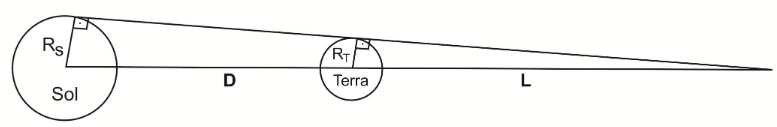
\includegraphics[scale=0.5]{img/2a.png}
            \end{figure}
            \begin{itemize}
                \item \textbf{Pergunta 2a) (0,5 ponto)} Calcule, em termos do raio da Terra ($R_T$) qual é o comprimento ($L$) da sombra  da  Terra,  mostrado  na  figura acima. Observação: $L$  é  medido  do  vértice  do  cone  de sombra até o centro da Terra.
                    \begin{itemize}
                        \item[$(\red{X})$] $L = 219,3 \cdot R_T$
                        \item[$(\quad)$] $L = 300,2 \cdot R_T$
                        \item[$(\quad)$] $L = 150 \cdot R_T$
                        \item[$(\quad)$] $L = 278,4 \cdot R_T$
                    \end{itemize}
                \item \textbf{Pergunta 2b) (0,3 ponto)} A  Lua cruza  o  cone  de  sombra  da  Terra  a uma distância $H = 60 \cdot R_T$. Calcule o raio ($d$) do cone de sombra nessa distância $H$, medido entre os centros da Terra e da Lua (não desenhada na figura), em função do raio da Terra ($R_T$).
                    \begin{figure}[H]
                        \centering
                        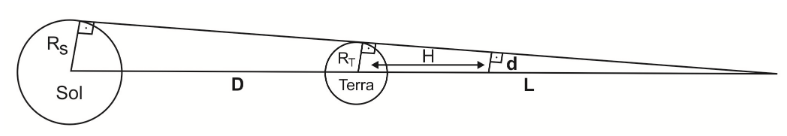
\includegraphics[scale=0.5]{img/2b.png}
                    \end{figure}
                    \begin{itemize}
                        \item[$(\red{X})$] $d = 0,73 \cdot R_T$
                        \item[$(\quad)$] $d = 1,5 \cdot R_T$
                        \item[$(\quad)$] $d = 0,25 \cdot R_T$
                        \item[$(\quad)$] $d = 2,77 \cdot R_T$
                    \end{itemize}
                \item \textbf{Pergunta 2c) (0,2 ponto)} Sabendo-se  que $R_T = 3.6 \cdot R_L$,  onde $R_L$ é o raio da Lua, calcule quantas vezes $d$ é maior do que $R_L$. Isso explica o porquê do eclipse lunar ser longo.
                    \begin{itemize}
                        \item[$(\red{X})$] $d = 2,63 \cdot R_L$
                        \item[$(\quad)$] $d = 3,14 \cdot R_L$
                        \item[$(\quad)$] $d = 1,36 \cdot R_L$
                        \item[$(\quad)$] $d = 2,15 \cdot R_L$
                    \end{itemize}
            \end{itemize}
        \item \textbf{Questão 3) (1 ponto)} Você deve ter ouvido falar dos satélites geoestacionários: aqueles que ficam sempre sobre o mesmo lugar na Terra (porque seu período para completar uma órbita é igual ao período de rotação da Terra). Esses satélites são muito úteis para transmitir sinais de televisão, rádio, telefonia, etc. \linebreak \linebreak Entretanto, para o sistema funcionar, as órbitas dos satélites estacionários devem ser todas próximas ao Equador. Logo, esses satélites não são bons para países muito ao norte ou muito ao sul. Por isso a Rússia desenvolveu um sistema diferente de satélites, chamados de Molniya. Trata-se de três satélites com órbitas bastante alongadas, como mostra a figura abaixo. \linebreak \linebreak Pelas Leis de Kepler, sabemos que a velocidade dos satélites é função da sua distância ao foco da elipse onde está a Terra. Dessa forma, próximo ao perigeu (o ponto mais próximo à Terra) o satélite vai passar rapidamente; próximo ao apogeu (o ponto mais distante da Terra), ele permanecerá por muito mais tempo. Assim, os astrônomos russos calculam a órbita para que o apogeu esteja por cima da Rússia. Além disso, eles colocam três satélites para que, a qualquer hora do dia, sempre haja pelo menos um satélite sobrevoando o território russo, para poder transmitir sinais. \linebreak \linebreak Considere o satélite Molniya da figura abaixo. Seu apogeu ($R_a$) está a $45.590 \, km$ do centro da Terra; seu perigeu ($R_p$), a $6.920 \, km$.
            \begin{figure}[H]
                \centering
                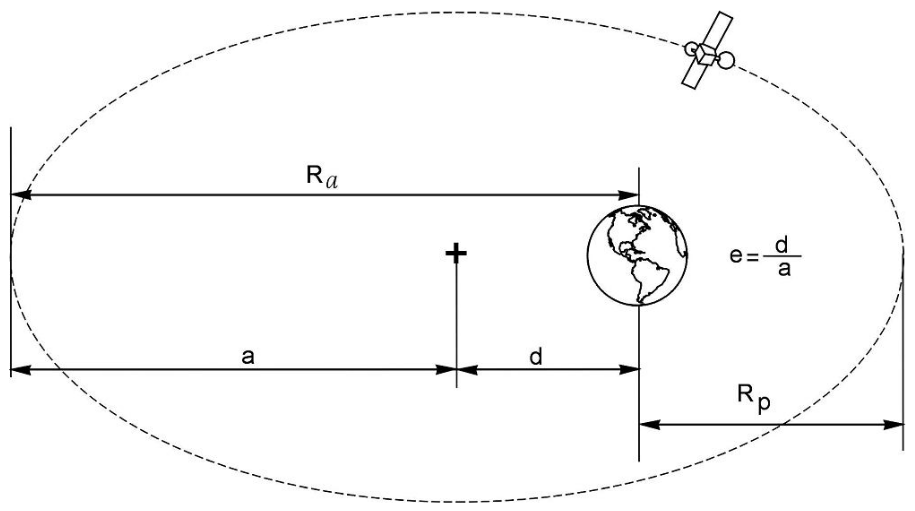
\includegraphics[scale=0.5]{img/3.png}
            \end{figure}
            \begin{itemize}
                \item \textbf{Pergunta 3a) (0,5 ponto)} Calcule o semi-eixo maior ($a$) da órbita.
                    \begin{itemize}
                        \item[$(\red{X})$] $a = 26.255 \, km$
                        \item[$(\quad)$] $a = 15.365 \, km$
                        \item[$(\quad)$] $a = 32.415 \, km$
                        \item[$(\quad)$] $a = 10.213 \, km$
                    \end{itemize}
                \item \textbf{Pergunta 3b) (0,5 ponto)} Calcule a excentricidade  ($e= \frac{d}{a}$) da órbita.
                    \begin{itemize}
                        \item[$(\red{X})$] $e = 0,74$
                        \item[$(\quad)$] $e = 0,23$
                        \item[$(\quad)$] $e = 0,95$
                        \item[$(\quad)$] $e = 1,24$
                    \end{itemize}
            \end{itemize}
    \end{itemize} \end{flushleft}

    \begin{flushright}
		\begin{large}
			Bons estudos!
		\end{large}
	\end{flushright}
\end{document}